%%=============================================================================
%% testen van de Automated reconnaissance tools
%%=============================================================================
% \chapter{Automated reconnaissance tools}
% \label{ch:Automated reconnaissance tools}

\chapter{\IfLanguageName{dutch}{tool evaluatie}{tool evaluatie}}
\label{ch:geautomatiseerde Reconnaissance}

\section{Methodology foor tool evaluatie}

De reconnaissance fase werdt uitgevoerd in een gecontroleerde virtuele omgeving (zie ~\ref{ch:Proof of Concept}) om de manuele en automatisatie tools te evalueren.
deze evaluatie is uitgevoerd met de OSSTMM framework nadruk op de Standaardiseren, Reproduceerbaar, Neutraal en Meetbare risico secties.
De manuele reconnaissance is uitgevoerd gebruik makende van 54 commando's, deze zijn gekozen om een zo bereed mogelijk oppervlakte te dekken van de reconnaissance fase verdeeld over 5 categorieën.
De automatisatie reconnaissance is uitgevoerd gebruik makende van 7 verschillende tools: AutoRecon, Cyberscan, LazyRecon, Sn1per, RustScan, Nuclei, ReconFTW.
Dit hoofdstuk zal een gedetailleerde vergelijking maken, kijkende naar de betrouwbaarheid, snelheid, bruikbaarheid, CPU gebruik en de OSSTMM RAV score.

% deze comanandos zijn uitgevoer in een gecontroleerde omgeving zie hoofdstuk ref{ch:PoC}, deze bieden ook een baselinen voor de evaluatie voor de geautomatiseerde tools.
% De manuele reconnaisansse is een belangerijk deel van deze bachelorproef.
% De manuele reconnaisanse is uitgevoerd voor de effectiviteiet van de individuele tools te testen binnen de OSSTMM framwork.
% Deze aanpak heb ik ondernomen door een zo breed moeglijke scala aan tools te gebruiken en met de informatie die er daar verzamleld werdt verder onderzocht im al de mogelijke kwetsbaarheden opn te leggen.
% Uit de manuele test is er een bash script opgesteld om de betroubaarheid van de tool, tijd en cpu gebruik te testen.
% In dit hooofdstuk zal de manuele reconnaisanse proces overlopen worden, categorisatie van 54 comanandos in 5 OSSTMM categorieen, de automatisatie van de 

\section{manuele reconnaissance}
De manuele reconnaissance werd uitgevoerd op Kali Linux 2024.2 (192.168.56.10) met doelwit Metasploitable2 (192.168.56.11) over een geïsoleerde virtuele netwerk (zie ~\ref{ch:Proof of Concept}).
Het uitvoeren van de manuele reconnaissance gebruikte 54 commando's, iedere commando is uitgekozen om ieder aspect van de reconnaissance te dekken wat gedefinieerd was in het OSSTMM Data network en Human secties (ref{tabel2}).
De commando's zijn manueel getest om de output, uitvoertijd en mogelijks foutmeldingen te verstaan, deze resultaten zijn opgeslagen in een Excel bestand(zie ~\ref{file:vergelijking_recon_manueel})
Na het uitvoeren van al de commando's is er een Bash script opgezet om de betrouwbaarheid van te tool, tijd, CPU gebruik te testen.

\subsection{categorisatie van de comanandos}

Om een structuur in reconnaissance te brengen zijn de 54 commando's georganiseerd in 5 categorieën, gebaseerd op hun functionaliteit en overeenkomst met de OSSTMM objectieven (Standaardiseren, Reproduceerbaar, Neutraal, Meetbare risico).
De categorieën zijn als volgt:

\begin{itemize}
  \item \textbf{Netwerk en host discovery} Geeft de actieve hosts en Netwerk configuraties.
    {\scriptsize \begin{itemize}
      \item \textmd{RAV score} V: hoog, A: laag, T: laag
    \end{itemize} }
  \item \textbf{poorten en service analyse} scans voor open poorten en lopende services
    \item {\scriptsize \begin{itemize}
      \item \textmd{RAV score} V: hoog, A: Medium, T: Low
    \end{itemize} }
  \item \textbf{web reconnaissance} Webservers en toepassingen weergeven. 
    {\scriptsize \begin{itemize}
      \item \textmd{RAV score} V: hoog, A: Medium, T: Medium
    \end{itemize} }
  \item \textbf{protocol en service enumiratie} Geeft specifieke protocollen en services weer.
  {\scriptsize \begin{itemize}
    \item \textmd{RAV score} V: Medium, A: hoog, T: hoog
  \end{itemize} }
  \item \textbf{vulnerability scanning} Detecteert mogelijke exploits en kwetsbaarheden.
  {\scriptsize \begin{itemize}
    \item \textmd{RAV score} V: hoog, A: hoog, T: Medium
  \end{itemize} }
\end{itemize}
  
\subsection{manuele uitvoer}
Deze commando's zijn manueel uitgevoerd, waar de output van de commando's zijn opgeslagen in de Excel sheet ~\ref{file:vergelijking_recon_manueel}.
De observaties zijn als volgt:

\begin{itemize}
  \item \textbf{Snelheid:} De uitvoer van de commando's varieert extreem van 0.06s naar 521s.
  \item \textbf{Betrouwbaarheid:} Sommige commando's falen door Metasploitable2 onstabiele services, wat voor betrouwbaarheidsprobemen kan zorgen.
  \item \textbf{Bruikbaarheid:} Interactieve commando's vragen manuele input, wat de uitvoer tijd en complexiteit moeilijker maken. Het gebruik en interpretatie van de tool hangt af van de ervaring en kennis van de pentester.
  \item \textbf{RAV score:} De RAV score is zeer variabel, dit geeft de betrouwbaarheid en de bruikbaarheid van de tool aan.

\end{itemize}

Deze manuele reconnaissance geeft hele goede en diepe inzichten in de werking van de Metasploitable2 en de verschillende services die er op staan.
Echter is dit een tijdrovend, repetetief, error gevoelig en staan de merendeel van de commando's niet in deze vergelijking doordat deze niet bruikbaar zijn voor deze specifieke case.

\subsection{bash script voor betroubaarheid}

Om de betrouwbaarheid te kunnen testen is er een bash script opgezet dat de 54 commando's bevat ~\ref{file:controle.sh}, dit om de betrouwbaarheid door consistentie te testen maar ook de error en time-out frequentie.
Dit script bevat:

\begin{itemize}
  \item \textbf{commando's organisatie} De commando's zijn georganiseerd in 5 verschillende categorieën, deze zijn opgeslagen in een matrix voor een modulaire uitvoering.
  \item \textbf{3x testen} De commando's zijn 3x uitgevoerd om de consistentie, tijd stabiliteit, error en time-out frequentie, en CPU gebruik te testen.
  \item \textbf{output structuur} De resultaten zijn opgeslagen in zijn categorie specifieke tekst bestand, hierin zit de commando output, tijd, CPU gebruik en error en time-out status.
  \item \textbf{interactieve commando's} De interactieve commando's werden vervangen door alternatieve niet-interactieve commando's, zo bekom je volledige automatisatie van het script. 
  \item \textbf{error handling} De errors en time-outs worden opgevangen en gelogd in een aparte tekst bestand.

\end{itemize}

\subsection{bash script uitvoer}

Deze uitvoer van de bash script zijn ingedeeld in 5 categorieën, Vulnerability Scanning, Protocol en Service Enumeratie, Poort en Service Analyse, Netwerk en Hostontdekking, Web Reconnaissance.
De meeste comanando's waren consistent over de 3 runs, met enkele uitzonderingen waar er inconsistentie en fouten optraden, wat wijst op een betrouwbare uitvoering binnen de virtuele omgeving.

De uitvoering van het bash script leverde de volgende resultaten:

\begin{itemize}
  \item \textbf{consistentie} de meeste commandos uit hetbach script zijn consistent over de drie runs, met enekele uitzonderingen waar er inconsistentie en fouten optraden.
  \item \textbf{Foutfrequentie} Een 10\% van al de comando's gaf een foutmelding of time-out, voornamelijk kwamen de meetse fouten voor bij de \textit{Vulnerability-scanning} en \textit{Protocol- en service-enumeratie} categorieën.
  \item \textbf{RAV score impact} De output consistentie bepaalt de RAV scores, een stabiele output vehoogt de \textit{Visibility}- en \textit{Access} scores.
  
\end{itemize}


De uitvoeringstijden en CPU verbruik werden ook berekend per categorie, door de totale tijd en CPU gebruik te nemen van alle commando's per categorie per run op te sommen en te delen over de 3 runs.

% 
% De uitvoeringstijden varieerden per categorie, met poort analyse en netwerk discovery als snelste (~7-37sec) en vulnerability scanning als meest tijdrovende (~37sec).
% De CPU verbruik schommeld veel van 0\% tot 104\% dit komt door dat de metingen gebreuren op de totale gebruik van alle cpu cores. waar de gemiddelde geberuik bij de categorie web reconnaissance het hoogst was (~46\%).


\begin{table}[h]
  \centering
  \footnotesize
  \begin{tabular}{lcc}
  \toprule
  \textbf{Categorie} & \textbf{Gemiddelde Uitvoeringstijd (per run)} & \textbf{Gemiddeld CPU-Gebruik} \\
  \midrule
  Vulnerability Scanning & $\sim$47 seconden & 17\% \\
  Protocol en Service Enumeratie & $\sim$7 seconden & 24\% \\
  Poort en Service Analyse & $\sim$37 seconden & 9\% \\
  Netwerk en Hostontdekking & $\sim$7 seconden & 36\% \\
  Web Reconnaissance & $\sim$7 seconden & 46\% \\
  \bottomrule
  \end{tabular}
  \caption{Gemiddelde uitvoeringstijd en CPU-gebruik per categorie}{\label{tab:cpu-uitvoeringstijd}}
\end{table}

\section{automatisatie reconnaissance}

De automatisatie van de reconnaissance fase is uitgevoerd met behulp van 7 verschillende tools.
Deze tools verzamelen verschillende taken als scanning, service enumeratie en vulnerability mapping in een herhaalbare workflow.
Ook al zijn deze tools krachtig kan niet iedere tool geschikt voor een gecontroleerde omgeving zonder internet toegang.
Deze tools die internet nodig hebben voor OSINT taken uit te voeren zoals Shodan, Spiderfoot, Amass en Recon-ng zijn uitgesloten van de volledige analyse maar worden wel erkend voor de volledigheid.

Iedere tool is onderzocht individueel en vergelijkend gebaseerd op technische gedrag, output kwaliteit en betrouwbaarheid, snelheid en OSSTMM RAV score.

Enkel de tools die volledig kunnen werken binnen in een lokaal netwerk zijn gebruikt.
Iedere tool werd geconfigureerd om de metasploitable2 te scannen, dit met de standaard of lichtelijke aanpassingen.
Alle data was verzameld voor de vergelijkende studie en een RAV score.

\subsection{AutoRecon}
Autorecon is een multi threaded enumiratie tool dat een grote varieatie heeft aan onderliggende scanning tools als Nmap, Feroxbuster, Nikto en meer.
Het detecteert automatisch open poorten,enumereert gelinkte services em verzameld relevante banners en metadata. 
Autorecon was getest in meerdere configuraites waaronder de single-target en full-port scans. 

scans aan elkaar hangt op basis van eerdere service discovery. 
Hier integreert AutoRecon tools als Nmap, Feroxbuster, Nikto en meer voor een volledige reconnaissance scan.

\begin{itemize}
  \item \textbf{Sterktes:} Hoge aanpasbaarheid, diepe integratie van meerdere tool, gestructureerde rapportering.
  \item \textbf{Limitaties:} Relatieve hoge uitvoeringstijd veroorzaakt door de uitgebreide scanning.
  \item \textbf{Uitvoeringstijd:} ~78 min
  \item \textbf{RAV score:}
    {\small
    \begin{itemize}
      \item \textbf{Visibility:} Hoog, haalde succesvol meerdere open poorten en servisce deatials. 
      \item \textbf{Access:} Medium, capabel om de  applicatie laag binnen te gaan en de specifieke service fingerprints identificeren. 
      \item \textbf{Trust:} Laag, geeft meerendeel publieke informatie zonder gevoelige credentials en bestanden bloot te leggen. 
    \end{itemize}
    } 
\end{itemize}

\subsection{cyberscan}

Cyberscan is een snelle en lichte scanner ontworpen om open poorten en services te identificeren. 
De voornaamste rol is de snelle enumiratie om de host beschikbaarheid en basis service te detecteren.

\begin{itemize}
  \item \textbf{Sterktes:} Zeer snel, efficient voor een eerdte verkenning.
  \item \textbf{Limitaties:} Mist diepte in de scans en heeft geen vulnerability detectie.
  \item \textbf{Uitvoeringstijd:} ~5 min
  \item \textbf{RAV score:}
    \small{
    \begin{itemize}
      \item \textbf{Visibility:} Medium, basis poort en protocol detectie.
      \item \textbf{Access:} Laag, heeft geen service fingerprinting og vulnerablility scanning gedaan.
      \item \textbf{Trust:} Geen, de output bevat geen gevoelige informatie. 
    \end{itemize}
    }
\end{itemize}

\subsection{Sn1per}
Sn1per is een volledige offensieve security scanner dat reconnaissance invoegt met vulnerablility scanning en rapportage. 
Deze tool presteerde gelijkaardig met AutoRecon maar geeft ook een gelimiteerde vulnerabilityanalyse zoals een standaard credential controles en openstaande admin interfaces.

\begin{itemize}
  \item \textbf{Sterktes:}Rijke features, gecombineerd met meerdere scanning fases in 1 uitvoer.
  \item \textbf{Limitaties:} Hogere systeem verbruik.
  \item \textbf{Uitvoeringstijd:} ~68 min
  \item \textbf{RAV score:}
    \small{
    \begin{itemize}
      \item \textbf{Visibility:}Hoog, gedetaileerde outputs aan poorten, services en http endpoints.
      \item \textbf{Access:}Medium, Heeft Standaard vulnerability controle.
      \item \textbf{Trust:} Medium, sommige zwakke configuraties en standaard instellingwn waren bloot gelegd.
    \end{itemize}
    }
\end{itemize}


\subsection{RustScan}

RustScan is geoptimaliseerd voor snelle poort scan's. 
Deze tool voert geen service enumeratie uit als standaard maar kan in samenwerking met Nmap werken. 

\begin{itemize}
  \item \textbf{Sterktes:} Buitengewone performatie, ieaal voor scannen van grote IP ranges.
  \item \textbf{Limitaties:} Heeft toegevoegde tools nodig voor de volledige functionaliteit. 
  \item \textbf{uitvoeringstijd:} <1 min
  \item \textbf{RAV score:}
    \small{
    \begin{itemize}
      \item \textbf{Visibility:} Hoog, deed een complete poort scan in slects enkele seconden.
      \item \textbf{Access:} Laag, staat niet in contact met services. 
      \item \textbf{Trust:} Geen, geeft geen contact met services.
    \end{itemize}
    }
\end{itemize}

\subsection{Nuclei}
Nuclei is een template gebaseerde scanner, gebruikt om gekende problemen zoals open panelen, misconfiguraite en verouderde software componenten.

\begin{itemize}
  \item \textbf{Sterktes:} Persizie scanning gebruik makende van comunity voorbeelden en makkelijk aanpasbaar.
  \item \textbf{Limitaties:} Niet geschikt voor standalone gebruik in reconnaissance.
  \item \textbf{uitvoeringstijd:} ~3 min
  \item \textbf{RAV score:}
    \small{
    \begin{itemize}
      \item \textbf{Visibility:}Laag, afhankelijk van eerder gekende enumeratie voor input. 
      \item \textbf{Access:} Medium, identificeert gekende kwetsbaarheden gebaseerd op de analyse.
      \item \textbf{Trust:} Hoog, capabel om verschillende misconfiguraties en gevoelige endpoints weer te geven.
    \end{itemize}
    }
\end{itemize}

\subsection{lazyRecon}
Lazyrecon is gemaakt om de reconnaissance makkelijker te maken door tools samen te zetten in een automatisatie script. 
In een internet gelimiteerde omgeving zijn de OSINT functionaliteiten uitgeschakeld, resulterende in een gelimiteerde capaciteit.

\begin{itemize}
  \item \textbf{Sterktes:} Simpele interface, integreerd meerdere tools.
  \item \textbf{Limitaties:} Sterk vertrouwen in online bronnen, offline functionaliteit is beperkt. 
  \item \textbf{uitvoeringstijd:} ~9 min
  \item \textbf{RAV score:}
    \small{
    \begin{itemize}
      \item \textbf{Visibility:} Medium, interne scan modules identificeren sommige lokale services en web applicaties.
      \item \textbf{Access:} Laag, geen mogelijkheid om meer geavanceerdere scans te doen door de offline staat.
      \item \textbf{Trust:} Geen, geen gevoelige data gedetecteert. 
    \end{itemize}
    }
\end{itemize}

\subsection{ReconFTW}

ReconFTW is een geavanceerde automatisatie tool gemakat voor een volledige reconnaissance. net zoals LazyRecon, veel van de de functionaliteiten zijn OSINT gebaseerd. 
Echter in de offline mode, geeft het nog steeds bruikbare scans binnenin de interne netwerk.

\begin{itemize}
  \item \textbf{Sterktes:} Groote functionaliteit bij internet-gebaseerde enumeratie.
  \item \textbf{Limitaties:} Grote limitatie offline.
  \item \textbf{uitvoeringstijd:} ~14 min
  \item \textbf{RAV score:} 
    \small{
    \begin{itemize}
      \item \textbf{Visibility:}Medium, onderzoekt toegangbaare servises en paginas.
      \item \textbf{Access:} Laag, verminderd door geen internet-gebaseerde enumeratie.
      \item \textbf{Trust:} Laag, minimale gevoelige informatie achterhaald. 
    \end{itemize}
    }
\end{itemize}

\section{resultatenanalyse}

De evaluatie van de tools is gebaseerd op betroubaarheid, Uitvoernelheid, bruikbaarheid, CPU gebruik en de RAV score. 
In dit deel wordt analyse ondersteund door een n staafdiagram dat de RAV-scores voor eleke tool visualiseert.  

\begin{figure}[H] 
\centering
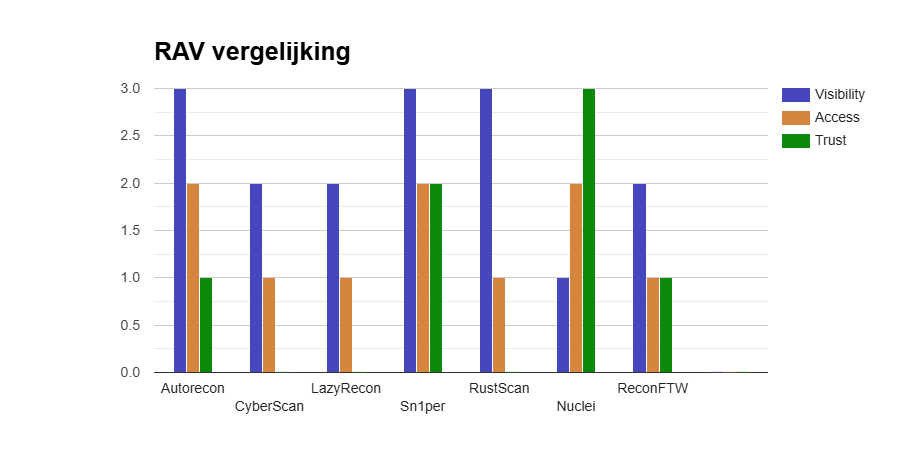
\includegraphics[width=\linewidth]{RAV_vergelijking.png}
\caption{RAV vergelijking per tool}
\label{fig:rav_barplot}
\end{figure}

Deze RAV score vergelijking laat zien dat geen enkele tool over al de 3 vakken uitsteekt. 
Autorecon en Sn1per geven de meest gebalanseerde resultaten, met een hoge Visibility en een gemidelde Access, deze goede resultaten komt te koste aan de een langere uitvoeringstijd en hogere CPU verbruik.
Rustscan is ongeonovertroffen in snelheid en poort scan's, terwijl Nuclei uitsteekt met zijn vulnerability detectie.
Cyberscan en Lazyrecon zijn op hun beurt ook geschikt voor snelle scans en ReconFTW ondaks de offline modus nog steeds mogelijk om bruikbare informatie te geven. 

uit deze resultaten zien we dat de automatisatie binnen de reconnaissance fase de efficiëntie verbeterd. 
Iedere automatisatie tool die in deze vergelijking aan bod is gekomen heeft zijn eigen use case, wat op zijn beurt dan ook weer speelt met de effectiviteit van de tools.
Voor deze studie met de focus op de reconnaissance fase en het zo veel mogelijk verzamelen van data zijn de AutoRecon en Sn1per de meest bruikbare door hun uitgebrijde analyse.

\section{vergelijking van manueel en geautomatiseerde reconnaissance}
De manuele en de automatisatie reconnaissance zijn vergeleken op basis van betrouwbaarheid, snelheid, bruikbaarheid en OSSTMM overeenkomst en RAV score.
\subsection{betroubaarheid}

\begin{itemize}
  \item \textbf{manuele reconnaissance} De manuele reconnaissance is betrouwbaar voor lichtere commando's, maar is kwetsbaar voor foutmeldingen in complexere commando's. De menselijke interpretatie van de output zorgt voor een compleet plaatje maar geeft ook een variabiliteit in de resultaten.
  \item \textbf{automatisatie reconnaissance} 
  \begin{itemize}
    \item \textbf{Autorecon, lazyRecon} Zeer betrouwbaar (90-95\%), occasionele errors met web scans.
    \item \textbf{recon-ng, Amass, theHarvester} Redelijk betrouwbaar (80-85\%) dit komende door de verschillende modules.
    \item \textbf{Shodan} Zeer betrouwbaar (90-95\%) maar niet volledig voor interne netwerken.
    \item \textbf{NetRecon, Cyberscan} Redelijk betrouwbaar (85\%).
  \end{itemize}
  \item \textbf{conclusie} De manuele aanpak is beter voor diepere scans maar is meer ondergevig aan fouten. De automatisatie tools zijn betrouwbaarder maar kunnen de diepgang van de manuele testen niet vervangen.
\end{itemize}

\subsection{snelheid}

\begin{itemize}
  \item \textbf{manuele reconnaissance} 2-3 Dagen voor de volledige reconnaissance fase, als dit uitgevoerd wordt door de bash script kan dit verminderen naar ~30 min. Echter vertelt dit niet het hele verhaal van de UItvoersnelheid,het merendeel van de tijd gaat naar het verstaan en interpreteren van de output.
  \item \textbf{automatisatie reconnaissance} 
  \begin{itemize}
    \item \textbf{Autorecon, lazyRecon, Cyberscan, NetRecon} 15-30 min
    \item \textbf{recon-ng, Amass, theHarvester} 5-20 min
    \item \textbf{Shodan} 5-10 min
  \end{itemize}
  \item \textbf{conclusie} De automatisatie tools zijn veel sneller dan de manuele reconnaissance, echter is dit niet volledig door de installatie en configuratie van de tools.
\end{itemize}


\subsection{bruikbaarheid}
\begin{itemize}
  \item \textbf{manuele reconnaissance} Vereist een grote kennis van de tools en de output, dit kan een probleem zijn bij minder ervaren pentesters.
  \item \textbf{automatisatie reconnaissance} 
  \begin{itemize}
    \item \textbf{Autorecon, lazyRecon, theHarvester} gebruiksvriendelijk en eenvoudig te gebruiken, maar de output kan moeilijker verstaanbaar zijn.
    \item \textbf{recon-ng, , Amass, Cyberscan} Redelijk kennis van de tool vereist.
    \item \textbf{Shodan, NetRecon} Simple en gebruiksvriendelijke interface.
  \end{itemize}
  \item \textbf{conclusie} De automatisatie tools zorgen er voor dat de barrière voor de kennis van de tools lager is.
\end{itemize}

\subsection{OSSTMM overeenkomst}
\begin{itemize}
  \item \textbf{Standaardiseren} Manueel is gestructureerd maar is afhankelijk van de kennis van de pentester; AutoRecon en lazyRecon hebben een makkelijke workflow en zijn gestructureerd.
  \item \textbf{Reproduceerbaar} Manueel is reproduceerbaar in een gecontroleerde omgeving; automatisatie zorgen orr meet consistentie.
  \item \textbf{Neutraal} Manueel en open source tools zijn neutraal, Shodan door eigen gegevens zorgt voor een lichte bias.
  \item \textbf{Meetbare risico} De RAV scores zorgen voor de meetbare risico's.
\end{itemize}



% \subsection{OSSTMM-Aligned Testing Protocol}

% \begin{itemize}
%   \item \textbf{Pre-Test fase}:
%   \begin{itemize}
%     \item defineer de Rules of Engagement (RoE) voor iedere tool.
%     \item geef securiy best practices aan.
%     \item configureer de testomgeving.
%   \end{itemize}
  
%   \item \textbf{Test Execution}:
%   \begin{itemize}
%     \item test de tool tegen Metasploitable 2.
%     \item documenteer iedere stap van de configuratie. 
%     \item documenteeer de systeem 
%     \item Monitored systeem gegevens (CPU, memory, netwerk)
%   \end{itemize}
  
%   \item \textbf{Post-Test analyse}:
%   \begin{itemize}
%     \item verzamel outputs en logs van de tools.
%     \item analyseer de resultaten.
%     \item berken de RAV score.
%   \end{itemize}
% \end{itemize}

% \section{tool evaluatie}

% \subsection{Network Scanning Suite}

% \subsubsection{Nmap Advanced Features}
% \begin{itemize}
%   \item \textbf{Scripting Engine}:
%   \begin{itemize}
%     \item 600+ NSE scripts categorized by:
%     \begin{itemize}
%       \item Discovery (35\%)
%       \item Vulnerability (25\%)
%       \item Exploit (15\%)
%       \item Miscellaneous (25\%)
%     \end{itemize}
%   \end{itemize}
  
%   \item \textbf{Performance Optimization}:
%   \begin{itemize}
%     \item Timing templates (-T0 to -T5)
%     \item Parallel scan algorithms
%     \item Adaptive host discovery
%   \end{itemize}
% \end{itemize}

% \begin{minted}[linenos,breaklines,frame=single]{bash}
% nmap -sV -sC -p- -T4 \
%      -oA scan_results \
%      target_ip
% \end{minted}





